\subsection{Voltage Level Detector With Hysteresis Applications:}

Once the circuit in Figure 3.5.0 were assembled, we started to increase and decrease the potentiometers resistance to visualize what does this circuit do. Finally we adjust the presets when the bulb went on and off appropriately, this means, when there were no "noise" ( oscillations ) in the bulb. This circuit were very similar that the one in figure 3.4.1, so, we measure the voltage in the photocell when there were no light and analogously, when there were light. This voltage values were registered in table 3.

\begin{figure}[H]
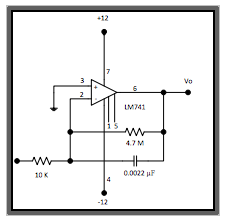
\includegraphics[width = 16.5cm, height = 8cm]{c6.png}
\centering \linebreak \linebreak Figure 3.5.0: Voltage level detector with hysteresis application
\end{figure} \hfill

\begin{center}
\begin{tabular}[.5cm]{c c c}
\toprule
\toprule
\hspace{200pt} & \hspace{100pt} $V_{i}$ \hspace{100pt}  \\
\midrule
\midrule
$V_{ref}$ & 7.5 V \\
\cmidrule{1-2}
Voltage in nR ( Voltage source turned off ) & 10.48 V \\
\cmidrule{1-2}
Photocell with light & 6.9 V \\
\cmidrule{1-2}
Photocell without light & 11.15 V \\
\bottomrule
\linebreak
\end{tabular}
\linebreak Table 3: Figure 3.5.0 voltage levels.
\end{center} \hfill

\pagebreak
